\documentclass[
	12pt,				% tamanho da fonte
	openright,			% capítulos começam em pág ímpar (insere página vazia caso preciso)
	oneside,			% para impressão em recto e verso. Oposto a oneside
	a4paper,			% tamanho do papel. 
	english,			% idioma adicional para hifenização
	french,				% idioma adicional para hifenização
	spanish,			% idioma adicional para hifenização
	brazil				% o último idioma é o principal do documento
	]{abntex2}

\usepackage{lmodern}			% Usa a fonte Latin Modern			
\usepackage[T1]{fontenc}		% Selecao de codigos de fonte.
\usepackage[utf8]{inputenc}		% Codificacao do documento (conversão automática dos acentos)
\usepackage{indentfirst}		% Indenta o primeiro parágrafo de cada seção.
\usepackage{color}				% Controle das cores
\usepackage{graphicx}			% Inclusão de gráficos
\usepackage{microtype} 			% para melhorias de justificação
\usepackage{transparent}
\usepackage{eso-pic}
\usepackage{amsthm,amsfonts}
\usepackage{float}
\usepackage{multirow}
\usepackage[table,xcdraw]{xcolor}
\usepackage{longtable}
\usepackage{lipsum}				% para geração de dummy text
%\usepackage[brazilian,hyperpageref]{backref}	 % Paginas com as citações na bibl
\usepackage[alf]{abntex2cite}	% Citações padrão ABNT
\usepackage{xcolor}
\usepackage{scalefnt}

\usepackage[font=small]{caption}     %% make caption in normal size
\usepackage{etoolbox}
\AtBeginEnvironment{longtabu}{\footnotesize}{}{}   %% change all longtabu content to foot note size

\definecolor{verde}{rgb}{0,0.5,0}
\usepackage{listings}
\lstset{
  language=C++,
  basicstyle=\ttfamily\small,
  keywordstyle=\color{blue},
  stringstyle=\color{verde},
  commentstyle=\color{red},
  extendedchars=true,
  showspaces=false,
  showstringspaces=false,
  numbers=left,
  numberstyle=\tiny,
  breaklines=true,
  backgroundcolor=\color{green!10},
  breakautoindent=true,
  captionpos=b,
  xleftmargin=0pt,
}


\titulo{Processo Agroindustrial de Processamento de Cacau}
\autor{Caio Henrique Silva Souza 99131\\Eduardo Favoretto Vale Bom 108139\\Gabriel Rodrigues Munhoz 106802\\João Vítor Batistão 108074}
\local{Maringá, PR}
\data{01.02.2022}
\orientador{}
\coorientador{}
\instituicao{%
  Universidade Estadual de Maringá - UEM
  \par
  Departamento de Engenharia de Produção - DEP}
\tipotrabalho{Tese (Doutorado)}
\preambulo{}

\definecolor{blue}{RGB}{41,5,195}

\makeatletter
\hypersetup{
     	%pagebackref=true,
	pdftitle={\@title}, 
	pdfauthor={\@author},
    	pdfsubject={\imprimirpreambulo},
	pdfcreator={LaTeX with abnTeX2},
	pdfkeywords={abnt}{latex}{abntex}{abntex2}{trabalho acadêmico}, 
	colorlinks=true,       		% false: boxed links; true: colored links
    	linkcolor=black,          	% color of internal links
    	citecolor=blue,        		% color of links to bibliography
    	filecolor=magenta,      		% color of file links
	urlcolor=blue,
	bookmarksdepth=4
}

\setlength{\parindent}{1.3cm}

\setlength{\parskip}{0.2cm}  % tente também \onelineskip

\makeindex

%\usepackage{fancyhdr}
%\fancyhead{}
%\fancyfoot{}
%\lhead{Processo Agroindustrial de Processamento de Cacau}
%\rhead{Processo Agroindustrial de Processamento de Cacau}

\AddToShipoutPicture{
\put(0,0){
\parbox[b][\paperheight]{\paperwidth}{%
\vfill
\centering
{\transparent{0.1}\includegraphics[scale=1.4]{../../Pictures/logoUEM.jpg}    }%
\vfill}}}



%\graphicspath{{../Pictures}}
\begin{document}

\begin{minipage}[c][0cm][c]{0cm} % a primeira minipágina tem uma altura de 1.5cm e uma largura de 3cm.

\centering


\includegraphics[scale=0.45]{../../Pictures/uem-modelo-04.png}  
\end{minipage}

\selectlanguage{brazil}

\frenchspacing 

% \pretextual

\imprimircapa


% ---
% RESUMOS
% ---

%\setlength{\absparsep}{18pt} % ajusta o espaçamento dos parágrafos do resumo
%\begin{resumo}
 
 
% \textbf{Palavras-chave}: latex. abntex. editoração de texto.
%\end{resumo}


% ---
% inserir o sumario
% ---
\pdfbookmark[0]{\contentsname}{toc}
\tableofcontents*
\cleardoublepage

% ----------------------------------------------------------
% ELEMENTOS TEXTUAIS
% ----------------------------------------------------------
\textual

\chapter{Introdução}
%\pagestyle{fancy}

\section{Contextualização do Tema}

O cacau é um fruto da espécie \textit{Theobroma cacao L.} que possui origem na região amazônica e seu uso, segundo arqueólogos equatorianos e franceses, já era realizado há cerca de 5.500 anos pelos povos amazônicos \cite{2}. No entanto, foi no século XVII que acabou se tornando um produto agrícola e cultivado em diferentes locais da América do Sul e Central devido a disseminação do cultivo pelos espanhóis, e posteriormente se expandindo aos poucos pelo mundo. \cite{1} 

Existem 6 principais produtos a partir do fruto de cacau: mel, polpa, nibs, chocolate, manteiga e cacau em pó, além da própria amêndoa do cacau e casca que também pode ser comercializada de uma forma menos processada. A maior parte desses produtos são voltados para o setor alimentício, no entanto é possível verificar aplicações também no setor cosmético e no setor de geração de energia. \cite{5}

Com mais da metade da produção nacional, 62$\%$, o sul da Bahia é a principal região produtora de cacau, seguida pela região norte do Brasil com 34$\%$ e o restante da produção, 4$\%$, espalhada pelo país \cite{1}. O Brasil é o 7º maior produtor do mundo e segundo o Instituto Brasileiro de Geografia Estatística (IBGE) o Brasil produziu em torno de 310 mil tonaledas. \cite{3} 


\section{Objetivos}

\subsection{Objetivo Geral}

Estudar o processamento de cacau na agroindústria, mais especificamente a produção de chocolate, abrangendo desde a parte normativa do setor, até o entendimento do mercado do produto em questão e as análises técnicas dos processos.

\subsection{Objetivos Específicos}

\begin{itemize}
\item Estudar o mercado, normas regulatórias, oportunidades e desafios do setor.
\item Realizar o mapeamento dos processos de uma produção de chocolate desde o recebimento do fruto até a embalagem, estoque e distribuição do produto final.
\item Calcular os balanços de massa e energia que são inerentes ao processo de produção.
\end{itemize}

\newpage
\chapter{Revisão Bibliográfica}
%\pagestyle{fancy}

%Este trabalho tem como foco um estudo de caso, que foi pautado em alguns processos estudados, são eles:
%Modelagem matemática, Simulação, Otimização e Controle de processos. Esses processos foram utilizados para melhor entendimento do funcionamento de um tanque de agitação que realiza a mistura de água com uma solução aquosa de hidróxido de sódio. 

%Para o desenvolvimento desse estudo, é de extrema importância entender minimamente o processo que será modelado, para que assim seja possível uma implementação prática que resulte em um resultado efetivamente assertivo e o mais próximo do real possível. Caso não exista o entendimento do tema proposto, a realização da modelagem matemática, da simulação do processo e por consequência a análise dos dados e a obtenção de otimizações fica totalmente imprecisa. 

\section{Histórico}

\subsection{História Mundial}

A árvore do cacau que se chama cacaueiro encontrou excelentes condições para o cultivo no território que hoje é conhecido como México há mais de 3.000 anos. Quem habitava o local naquela época era a civilização dos Olmecas, mas após o desaparecimento de tal civilização, os Maias que foram para essa área e utilizavam o cacau para produção de bebidas amplamente utilizadas em rituais. \cite{7}

Farrow (2005) comenta que 600 a.c. os próprios Maias implementaram as primeiras plantações de cacau em Yucatan e na Guatemala. \cite{7}

O chocolate era uma amplamente consumido por vários povos pré-colombianos, Maias, Incas e Astecas produziam amplamente, porém os incas chegaram ao nível de produzir em escala a ponto de ser suficiente para toda população, já com os Maias e Astecas só a nobreza tinha tal privilégio. 

\subsection{Chegada do cacau na Europa}

No ano de 1502, com a chegada de Cristóvão Colombo nas américas, houve o primeiro contato europeu com o cacau, quando um chefe asteca presenteou os marinheiros de Cristóvão com a bebida. No entanto era uma bebida amarga e picante e o europeu não deu a mínima importância. \cite{7}

O produto foi realmente trazido para a Europa quando o Espanhol Hernando Cortez chegou no México com o intuito de conquistar as terras, porém o povo Asteca os recebeu com cordialidade por acreditarem ser uma reencarnação. Com isso, foi possível a troca e o conhecimento das tradições dos astecas pelos Espanhóis e o cacau/chocolate. Tal especiaria foi levada para a europa e amplamente explorado para fins comerciais e entre os dois povos. \cite{7}

Neste momento, o chocolate era altamente utilizado pela nobreza juntamente com mel para amenizar o amargor. Tal bebida era extremamente utilizada pela realeza e nobreza, sendo uma das principais bebidas e mais utilizadas na região, porém somente na Espanha.

Em meados de 1615 o casamento entre o françes Luís XIII com a infanta Espanhola confirmou a adoção do produto também na França que passou a fazer parte da corte.

\subsection{Cacau no Brasil}

No Brasil a chegada do cacau se deu no século XVIII na Bahia e com o clima propício para a produção do cacaueiro a região rapidamente se tornou produtora do cacau, produzindo mais de 300 mil toneladas ao ano. \cite{1} \cite{7}

Segundo Lima, 2008 outros estados como o Pará e Rondônia são produtores de cacau até os dias atuais.

Segundo os dados do último Censo Agropecuário (2017), Há mais de 93 mil estabelecimentos produtores de cacau no País, sendo 69 mil na Bahia (74$\%$ do total) e 18 mil no Pará (19$\%$). Em 2019 o Brasil já alcançava a marca de mais de 250 mil toneladas produzidas como consta na figura \ref{fig2}. \cite{7}

\begin{figure}[H]
\begin{center}
\caption{Desempenho do Brasil em 2019 na atividade agrícola do cacau}
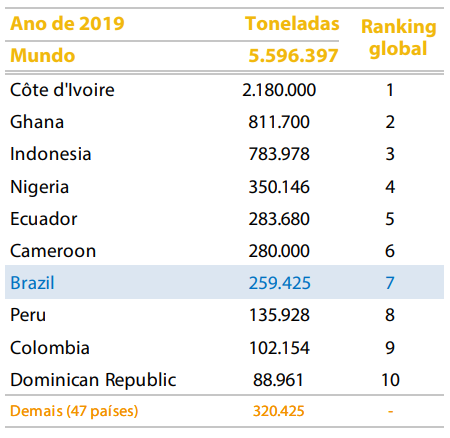
\includegraphics[scale=0.8]{../../Pictures/tabela.png} 
\label{fig2}
\legend{Fonte: \cite{8}}
\end{center}
\end{figure}

No Brasil o cultivo gera mais de 269 mil empregos diretos.

Segundo os dados do Ministério da Agricultura, a lavoura da amêndoa gerou R$\$$ 3,8 bilhões de valor bruto da produção agrícola (VBPA) em 2020, segundo os dados do Ministério da Agricultura, Pecuária e Abastecimento (MAPA). Os estados do Pará e da Bahia representaram 94$\%$ desse total. \cite{8}

\subsection{Dados Atuais}

A produção global de cacau atual é de aproximadamente 4.84M de toneladas, sendo a o continente africano o líder da produção 	com um market share de 76,1$\%$. \cite{8}

O Brasil é o sétimo maior produtor de cacau do mundo, sendo uma produção anual de 259.425 toneladas.

Segundo os dados do último Censo Agropecuário (2017), Há mais de 93 mil estabelecimentos produtores de cacau no País, sendo 69 mil na Bahia (74$\%$ do total) e 18 mil no Pará (19$\%$). \cite{8}

No Brasil o cultivo gera mais de 269 mil empregos diretos.

Segundo os dados do Ministério da Agricultura, a lavoura da amêndoa gerou R$\$$ 3,8 bilhões de valor bruto da produção agrícola (VBPA) em 2020, segundo os dados do Ministério da Agricultura, Pecuária e Abastecimento (MAPA). Os estados do Pará e da Bahia representaram 94$\%$ desse total. \cite{8}


\subsection{Avanços do processamento}

Antigamente o cacau era um privilégio da nobreza, porém atualmente com o avanço da tecnologia no processamento, o cacau se tornou amplamente utilizado pelo mundo todo. \cite{9}

Técnicas como a Conchagem (os ingredientes refinados recebem mais adição de gordura e emulsificante, formando uma massa fluida) e os maquinários possibilitaram a expansão da produção do chocolate. \cite{9}

\section{Matéria-prima}

O presente estudo tem como foco entender o processo de fabricação de chocolate através do cacau como matéria-prima. Analisando alguns dados sobre o cacau no mundo e no Brasil é possível afirmar que esse setor é muito promissor.

Atualmente a lavoura ocupa uma área de 617,5 mil hectares no País, e produz cerca de 310,5 mil toneladas, segundo o Instituto Brasileiro de Geografia e Estatística (IBGE). A maior área de plantio está na Bahia, com 440 mil hectares, 71,2$\%$ da área de cacau no País, o Pará é o maior produtor, com 146,4 mil toneladas numa área de 149,8 mil hectares. A produção baiana, por sua vez, é de 106 mil toneladas. Juntos somam 93$\%$ da produção nacional. \cite{6}

Uma das causas da grande produção dessa matéria-prima no país é o ambiente favorável, o cacaueiro (\textit{Theobroma cacao}) é uma frutífera tropical, originada da região amazônica.

Em relação aos métodos de produção do cacau foram identificados seis técnicas diferentes, e variações em dois desses métodos (Tabela \ref{table1}). Esses métodos apresentam uma gradação entre o plantio completamente exposto ao sol (corte e queima) até aquele contendo um sombreamento denso (cabruca). A categoria ‘outros métodos’ reúne os de menor relevância em termos de área cultivada e, por isso, não foi incluída na Tabela \ref{table1}. Esses seis métodos são descritos a seguir em seus respectivos contextos históricos, o que permite compreender sua origem e tentativa de diferenciação em relação às práticas correntes no momento da nova propositura. Assim, apresentam-se subdivididos em dois grandes períodos, caracterizados como o início de implantação da cacauicultura e o período de sua expansão e intensificação. \cite{10}

{\fontsize{5.8}{8}\selectfont
\begin{center}
\begin{longtable}[c]{c|c|c|c|c}
\caption{Principais métodos de implantação e manejo dos cacauais, seus procedimentos, vantagens e desvantagens.}
\label{table1}\\
\hline
\rowcolor[HTML]{EFEFEF} 
\textbf{\begin{tabular}[c]{@{}c@{}}Método \\ e suas variações\end{tabular}} &
  \textbf{\begin{tabular}[c]{@{}c@{}}Período provável \\ de implantação \\ do método\end{tabular}} &
  \textbf{\begin{tabular}[c]{@{}c@{}}Procedimentos\\ efetuados\end{tabular}} &
  \textbf{Vantagens} &
  \textbf{Desvantagens} \\ \hline
\endhead
%
Corte e queima &
  1746 &
  \begin{tabular}[c]{@{}c@{}}Corte de toda a vegetação\\ nativa, seguido da queima.\\ As sementes de cacau eram\\ plantadas diretamente no\\ campo sob a sombra de cultivos\\ temporários, como mandioca\\ e milho. Após a colheita, as\\ plantas de cacau eram mantidas\\ sem o sombreamento até que\\ surgissem árvores espontâneas\\ na área. Após sete a dez anos, o\\ sombreamento era removido e a\\ plantação, mantida a pleno sol\end{tabular} &
  \begin{tabular}[c]{@{}c@{}}Elevada \\ produtividade\\ nos primeiros \\ anos\end{tabular} &
  \begin{tabular}[c]{@{}c@{}}Destruição das substâncias\\ húmicas do solo; estresse\\ das jovens plantas de cacau\\ sem o sombreamento;\\ vigorosa emergência\\ de plantas espontâneas;\\ elevada demanda de\\ mão de obra; rápido\\ envelhecimento da\\ plantação\end{tabular} \\ \hline
\begin{tabular}[c]{@{}c@{}}Corte sem\\ queimada\\ (Variação do\\ método corte e\\ queima)\end{tabular} &
  \begin{tabular}[c]{@{}c@{}}Primeiras décadas\\ de 1900\end{tabular} &
  \begin{tabular}[c]{@{}c@{}}Os mesmos procedimentos\\ do método de corte e queima\\ eram efetuados, com exceção\\ da queimada da vegetação\\ derrubada\end{tabular} &
  \begin{tabular}[c]{@{}c@{}}Conservação\\ de substâncias\\ húmicas do solo\end{tabular} &
  \begin{tabular}[c]{@{}c@{}}A vegetação cortada\\ deixada no solo \\ atrapalhava a movimentação \\ dos trabalhadores\end{tabular} \\ \hline
Cabruca tradicional &
  \begin{tabular}[c]{@{}c@{}}Primeiras décadas\\ de 1900\end{tabular} &
  \begin{tabular}[c]{@{}c@{}}Corte da vegetação herbácea\\ e do estrato intermediário.\\ Raleamento da vegetação do\\ dossel dominante, poupando-se\\ do corte as árvores de maior\\ porte, com copa alta e folhagem\\ pouco densa. Na fase adulta\\ dos cacaueiros, raleava-se o\\ sombreamento por meio de\\ anelamento das árvores\end{tabular} &
  \begin{tabular}[c]{@{}c@{}}Conservação\\ de substâncias\\ húmicas do solo;\\ controle de plantas\\ espontâneas; rápido\\ desenvolvimento\\ dos cacaueiros;\\ conservação da\\ sociobiodiversidade;\\ economia em mão\\ de obra\end{tabular} &
  \begin{tabular}[c]{@{}c@{}}Queda de folhas, galhos\\ e árvores mortas sobre\\ os cacaueiros, podendo\\ danificá-los; baixa\\ produtividade\end{tabular} \\ \hline
\begin{tabular}[c]{@{}c@{}}Cabruca mantida\\ apenas no\\ sombreamento\\ provisório\\ (Variação do\\ método cabruca\\ tradicional)\end{tabular} &
  \begin{tabular}[c]{@{}c@{}}Primeiras décadas\\ de 1900\end{tabular} &
  \begin{tabular}[c]{@{}c@{}}Os mesmos procedimentos\\ do método cabruca tradicional\\ eram efetuados para a\\ formação do sombreamento. O\\ sombreamento era removido\\ após alguns anos do plantio dos\\ cacaueiros, ainda durante a fase\\ juvenil\end{tabular} &
  \begin{tabular}[c]{@{}c@{}}Conservação de\\ substâncias húmicas\\ do solo durante a fase\\ juvenil dos cacaueiros;\\ maior produtividade\\ dos cacaueiros\end{tabular} &
  \begin{tabular}[c]{@{}c@{}}Estresse das jovens\\ plantas de cacau sem o\\ sombreamento; rápido\\ envelhecimento da\\ plantação\end{tabular} \\ \hline
\begin{tabular}[c]{@{}c@{}}Intermediário\\ entre corte e\\ queima e cabruca\end{tabular} &
  \begin{tabular}[c]{@{}c@{}}Primeiras décadas\\ de 1900\end{tabular} &
  \begin{tabular}[c]{@{}c@{}}Derrubava-se a mata, poupando\\ do corte um número menor de\\ árvores em relação ao método\\ cabruca\end{tabular} &
  \begin{tabular}[c]{@{}c@{}}Fornecia\\ imediatamente o\\ sombreamento\\ definitivo, sem a\\ necessidade de\\ raleamentos futuros\end{tabular} &
  \begin{tabular}[c]{@{}c@{}}Queda de galhos mais\\ frequente em relação ao\\ que ocorre com a cabruca,\\ pois as árvores isoladas\\ eram menos resistentes ao\\ vento\end{tabular} \\ \hline
Derruba total &
  1964 &
  \begin{tabular}[c]{@{}c@{}}Roçagem da vegetação rasteira\\ e de toda a vegetação arbórea\\ nativa. Após 30-60 dias, efetuava-se \\ a queima da vegetação abatida.\\ Plantio de mudas de bananeira\\ para formação do sombreamento\\ provisório e de mudas de espécies\\ do gênero Erythrina para formação\\ do sombreamento definitivo,\\ com espaçamento de 24 x 24 m\\ (densidade de 25-30 árvores de\\ sombra por hectare)\end{tabular} &
  \begin{tabular}[c]{@{}c@{}}Elevada produtividade\\ nos primeiros anos de\\ cultivo\end{tabular} &
  \begin{tabular}[c]{@{}c@{}}Envelhecimento precoce\\ das plantações; entrada\\ em produção tardia; maior\\ custo de implantação\\ (quatro vezes mais caro em\\ comparação ao método\\ cabruca tradicional)\end{tabular} \\ \hline
\begin{tabular}[c]{@{}c@{}}Cabruca\\ tecnicamente\\ formada\end{tabular} &
  1978 &
  \begin{tabular}[c]{@{}c@{}}Execução das operações culturais\\ de acordo com os mesmos\\ critérios recomendados para\\ o método derruba total, com\\ exceção do preparo da área e do\\ raleamento do sombreamento.\\ A densidade do sombreamento\\ definitivo é de 25-30 árvores de\\ sombra por hectare\end{tabular} &
  \begin{tabular}[c]{@{}c@{}}Reduzida demanda\\ em capital, mão\\ de obra para a\\ implantação do\\ cacaual (economia\\ de 30\%) e tempo\\ na formação do\\ cacaual\end{tabular} &
  \begin{tabular}[c]{@{}c@{}}Queda de árvores\\ mortas e galhos sobre\\ os cacaueiros devido ao\\ raleamento\end{tabular} \\ \hline
\begin{tabular}[c]{@{}c@{}}Consórcio \\ cacau-seringueira\end{tabular} &
  \begin{tabular}[c]{@{}c@{}}Década de \\ 1980\end{tabular} &
  \begin{tabular}[c]{@{}c@{}}Plantio de cacaueiros nas\\ entrelinhas das seringueiras,\\ originalmente estabelecidas no\\ espaçamento de 7 x 3 m, com\\ densidade de aproximadamente\\ 450 cacaueiros por hectare\end{tabular} &
  \begin{tabular}[c]{@{}c@{}}As receitas econômicas\\ provenientes\\ da heveicultura\\ complementam as \\ receitas provenientes \\ da venda das \\ amêndoas de cacau\end{tabular} &
  \begin{tabular}[c]{@{}c@{}}Manejo das copas das\\ seringueiras de difícil\\ execução e custo elevado.\\ Pode haver sombreamento\\ excessivo para os\\ cacaueiros\end{tabular}
\end{longtable}
\centering \footnotesize{Fonte: \cite{10}}
\end{center}
}

\section{Produto}

\subsection{Importância Nutricional}
Segundo a Unimed \cite{unimed}, alguns benefícios podem ser elencados quando se fala do chocolate e esses são:

\begin{itemize}
\item O chocolate proporciona uma grande sensação de bem-estar
\item O consumo moderado de chocolate melhora o fluxo arterial 
\item Seu alto poder hidratante torna-o queridinho também no setor estético
\item Contribui para a saúde cerebral, reduzindo danos de acidente vascular cerebral
\item Reduz o estresse e alivia dores 
\item Melhora a saúde do coração
\item Estimula o sistema nervoso central
\item Diminui a sensação arterial
\item Protege a pele do sol
\item Diminui a fome
\end{itemize}

Mas pode-se elencar os benefícios por tipo de chocolate, o chocolate ao leite, chocolate meio amargo e amargo e chocolate branco.

O chocolate meio amargo e amargo são ótimos na circulação sanguínea, aumentam o colesterol bom, além de ser muito rico em alguns nutrientes, tais como o magnésio, ferro e selênio. O consumo moderado diário deste tipo de chocolate aumenta o metabolismo e reduz o apetite. \cite{saude}
	
Já o chocolate é o chocolate que tem menos gordura hidrogenada e por isso é o menos calórico.
	
Por fim, o chocolate branco tem uma característica principal de ter menos cafeina na sua composição e por oferecer mais energia ao corpo. \cite{saude}

% Please add the following required packages to your document preamble:
% \usepackage[table,xcdraw]{xcolor}
% If you use beamer only pass "xcolor=table" option, i.e. \documentclass[xcolor=table]{beamer}
% \usepackage{longtable}
% Note: It may be necessary to compile the document several times to get a multi-page table to line up properly
\begin{longtable}[c]{
>{\columncolor[HTML]{EFEFEF}}l |l|l}
\caption{Informações nutricionais do chocolate ao leite - 25g}
\label{table3}\\
\textbf{} & \cellcolor[HTML]{EFEFEF}\textbf{Quantidade por porção} & \cellcolor[HTML]{EFEFEF}\textbf{\% Valor diário} \\ \hline
\endhead
%
\textbf{Valor energético}   & 134 kcal  & 26,8 \% \\ \hline
\textbf{Carboidrato}        & 15 g      & 20,0 \%   \\ \hline
\textbf{Proteína}           & 1,2 g     & 6,4 \%  \\ \hline
\textbf{Gorduras totais}    & 7,7 g    & 56,0 \%   \\ \hline
\textbf{Gorduras saturadas} & 4,4 g    & 80,0 \%   \\ \hline
\textbf{Sódio}              & 11 mg     & 1,8 \% \\ \hline
\textbf{Colesterol}                  & 5,36 mg  &   0,9 \%  \\ \hline
\textbf{Fibra alimentar}             & 0,7 g     & 11,2 \% \\ \hline
\textbf{Cálcio}                      & 44,64 mg & 17,8 \% \\ \hline
\textbf{Ferro}                       & 0,36 mg   & 7,9 \% 
\end{longtable}
\begin{center}
\footnotesize{Fonte: \cite{fatsecret}}
\end{center} 
% Please add the following required packages to your document preamble:
% \usepackage[table,xcdraw]{xcolor}
% If you use beamer only pass "xcolor=table" option, i.e. \documentclass[xcolor=table]{beamer}
% \usepackage{longtable}
% Note: It may be necessary to compile the document several times to get a multi-page table to line up properly
\begin{longtable}[c]{
>{\columncolor[HTML]{EFEFEF}}l |l|l}
\caption{Informações nutricionais do chocolate meio amargo - 25g}
\label{table4}\\
\textbf{}                 & \cellcolor[HTML]{EFEFEF}\textbf{Quantidade por porção} & \cellcolor[HTML]{EFEFEF}\textbf{\% Valor diário} \\ \hline
\endhead
%
\textbf{Valor energético} & \cellcolor[HTML]{FFFFFF}131 kcal                       & \cellcolor[HTML]{FFFFFF}7\%                      \\ \hline
\textbf{Carboidrato}        & 14 g  & 5,0 \%  \\ \hline
\textbf{Proteína}           & 2 g   & 4,0 \%  \\ \hline
\textbf{Gorduras totais}    & 8,3 g & 15,0 \% \\ \hline
\textbf{Gorduras saturadas} & 5,4 g & 24,0 \% \\ \hline
\textbf{Sódio}              & 12 mg & 1,0 \%  \\ \hline
\textbf{Gorduras trans}              & 0 mg  &   -    \\ \hline
\textbf{Fibra Alimentar}             & 2 g   & 6,0 \%  \\ \hline
\textbf{Cálcio}                      & 35 mg & 4,0 \%  \\ \hline
\end{longtable}
\begin{center}
\footnotesize{Fonte: \cite{fatsecret}}
\end{center} 
% Please add the following required packages to your document preamble:
% \usepackage[table,xcdraw]{xcolor}
% If you use beamer only pass "xcolor=table" option, i.e. \documentclass[xcolor=table]{beamer}
% \usepackage{longtable}
% Note: It may be necessary to compile the document several times to get a multi-page table to line up properly
\begin{longtable}[c]{
>{\columncolor[HTML]{EFEFEF}}l |l|l}
\caption{Informações nutricionais do chocolate amargo - 25g}
\label{table5}\\
\textbf{}        & \cellcolor[HTML]{EFEFEF}\textbf{Quantidade por porção} & \cellcolor[HTML]{EFEFEF}\textbf{\% Valor diário} \\ \hline
\endhead
%
\textbf{Valor energético} & \cellcolor[HTML]{FFFFFF}131 kcal              & \cellcolor[HTML]{FFFFFF}7\%             \\ \hline
\textbf{Carboidrato}              & 13 g    & 4,0 \%   \\ \hline
\textbf{Proteína}                 & 2 g     & 3,0 \%   \\ \hline
\textbf{Gorduras totais}          & 9,2 g   & 17,0 \%  \\ \hline
\textbf{Gorduras saturadas}       & 5,8 g   & 26,0 \%  \\ \hline
\textbf{Sódio}                    & 5 mg    & 0,4 \% \\ \hline
\textbf{Gorduras trans}  & 0 mg    &    -    \\ \hline
\textbf{Fibra Alimentar} & 3 g     & 9,0 \%   \\ \hline
\textbf{Cálcio}          & 12,5 mg & 8,0 \%   \\ \hline
\end{longtable}
\begin{center}
\footnotesize{Fonte: \cite{fatsecret}}
\end{center} 

\subsection{Importância Ambiental}

A produção do cacau vem se tornando cada vez mais ESG com o tempo, dados da ONU dizem que houve um aumento de 8$\%$ na produção sustentável dos grãos de cacau entre 2017 e 2018, ou seja, a produção sustentável saiu de  36$\%$ em 2017 para 44$\%$ em 2018. \cite{xpeed}

Ao mesmo tempo, a indústria do chocolate também vem aumentando o direcionamento ESG com o tempo. Com as certificações de qualidade atualizadas, é possível saber qual produtor e fabricante tem um pensamento e uma produção sustentável ou não, com a ISO 9001:2015 é fácil realizar essa diferenciação. \cite{dengo}

\subsection{Importância Cultural}

A importância cultural do cacau se resume em 3 tópicos, são eles: o econômico, o histórico e o local.

Sobre a história do cacau, já foi abordado acima na introdução.

Sobre a importância de localização: O cacaueiro é uma planta nativa das bacias do rio Amazonas e rio Orinoco e tem a sua origem nas américas central e do sul. Para muitos povos havia até uma importância religiosa, como os Astecas. \cite{1}

Os próprios índios torravam e trituravam o fruto entre pedras para produzir um tipo de bebida típica, além disso, no Brasil, os maiores produtores do cacau estão localizados principalmente na Bahia e Pará, foi na Bahia que o cacau foi levado em meados do século XVIII. \cite{7}

Sobre a economia do cacau: No Brasil, o cacau é produzido em sua maioria em larga escala, sendo médios e grandes produtores. A concentração da produção se encontra principalmente na Bahia, Pará, Rondônia e Espírito Santo pelas características climáticas principalmente. No entanto, historicamente já passou por várias crises causando a redução da produção interna. \cite{8}

\newpage
\chapter{Mercado}
%\pagestyle{fancy}

Segundo a Associação Brasileira da Indústria de Chocolates, Amendoim e Balas (ABICAB). o brasileiro consumiu em 2020 11 bilhões de reais em chocolate, um crescimento de 1,5$\%$ comparado ao ano anterior. O presidente da associação, Ubiracy Fonseca, defende que a indústria de chocolates apresentou resultados muito consistentes para um ano tão atípico como foi 2020, e que os indicadores desse mercado apresentam potencial significativo para o crescimento do consumo interno e externo do setor. \cite{4}

\begin{figure}[H]
\begin{center}
\caption{Balança comercial de vendas de chocolates do Brasil em milhões de dolares}
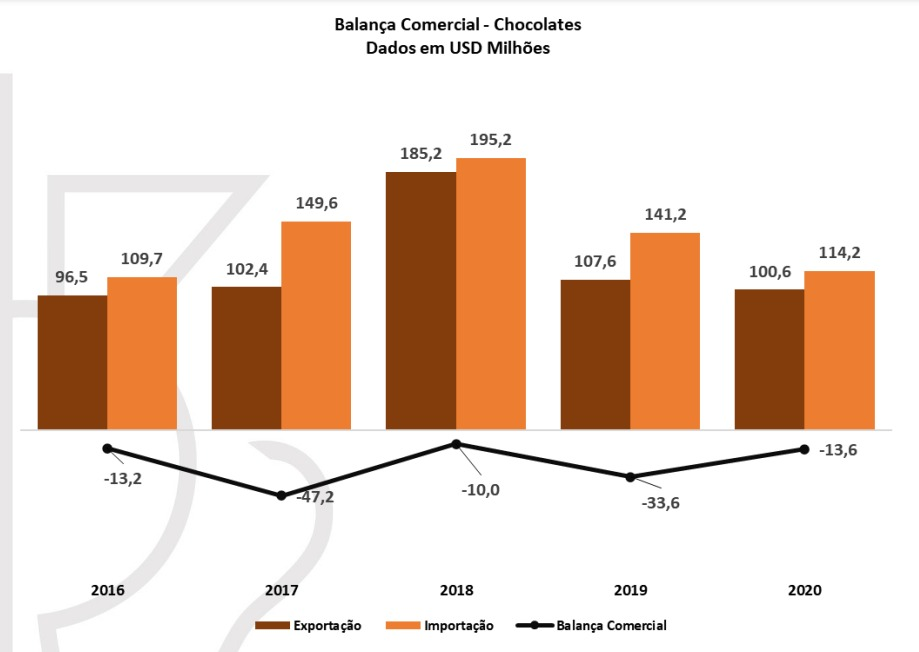
\includegraphics[scale=0.4]{../../Pictures/fig2.jpeg} 
\label{figmercado}
\legend{Fonte: \cite{4}}
\end{center}
\end{figure}

Analisando os números da KPMG, é possível concluir que a balança comercial do mercado de chocolate no brasil opera no negativo, ou seja, para que seja suprida a necessidade de chocolate no nosso país, foi importado 13 milhões de dólares a mais do que os valores de nossa exportação. Isso se dá pela falta de transformação da matéria prima em produto acabado levando em consideração que o país é o sétimo maior produtor de cacau do mundo. Esse número ainda é o menor dos últimos 5 anos, o que mostra que nossa indústria está em ascensão. \cite{forbes}

O chocolate ainda está presente em 82,6$\%$ dos lares brasileiros, um aumento de 9$\%$ percentuais comparado ao ano anterior. O avanço no consumo dos lares, juntamente com a grande necessidade de importação, resultou no aumento da produção de chocolate no último ano. \cite{4}

\begin{figure}[H]
\begin{center}
\caption{Gráfico comparativo entre produção, exportação e importação em volume}
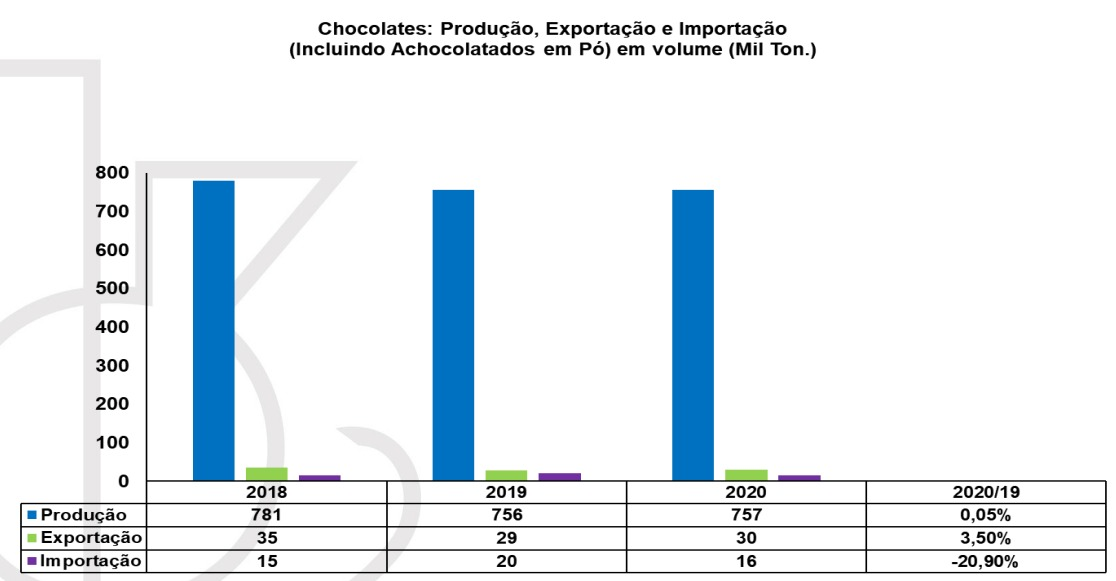
\includegraphics[scale=0.4]{../../Pictures/fig1.jpeg} 
\label{figmercado2}
\legend{Fonte: \cite{4}}
\end{center}
\end{figure}

\newpage
\chapter{Normas e Leis Regulamentadoras}
%\pagestyle{fancy}

O setor alimentício possui leis e normas bem definidas e detalhadas pela Agência Nacional de Vigilância Sanitária (Anvisa). Essa organização, segundo artigo 8º da Lei n. 9782/99 \cite{anvisa9782}, deve: “regulamentar, controlar e fiscalizar os produtos e serviços que envolvam risco à saúde pública”. Então será principalmente por meio dela que a empresa deve se informar para que esteja condizente com a legislação e normas vigentes. 

A principal preocupação desse setor é com relação às condições higiênicos-sanitárias, pois engloba todo o processo de fabricação, desde o recebimento das matérias-primas até o transporte final do produto acabado. Logo, a empresa deve se atentar principalmente à PORTARIA Nº 326 postada em 1997 \cite{anvisa326} que menciona o seguinte objetivo: “O presente Regulamento estabelece os requisitos gerais (essenciais) de higiene e de boas práticas de fabricação para alimentos produzidos/fabricados para o consumo humano.” 

Além disso, é importante estar de acordo com a legislação e os projetos de lei que existem para criação do produto, para planejar sua composição e marca e que consiga atender a todos os requisitos e possa ser comercializado sem problemas. Nesse sentido, os produtos que serão comercializados pela empresa são: chocolate amargo, chocolate meio-amargo e chocolate ao leite que devem obedecer a RESOLUÇÃO DE DIRETORIA COLEGIADA - RDC N° 264, de 2005 \cite{anvisa264}. Contudo, já existe o Projeto de Lei n° 1769, de 2019 \cite{anvisa1769} que pode influenciar nos requisitos relacionados à composição do chocolate.  

Por fim, ainda existem os requisitos relacionados ao modo como o produto será embalado e detalhes que necessitam estar nos rótulos de cada produto. Segundo a RESOLUÇÃO DE DIRETORIA COLEGIADA - RDC Nº 91, de 2001 \cite{anvisa91}, as embalagens, da mesma forma que os equipamentos que entram em contato com alguma parte do produto, devem manter o alimento protegido de fatores externos e não podem interferir ou mudar suas características. Existe uma classificação de embalagens de acordo com o tipo de material que é utilizado, e cada um deles possui um regulamento específico. Os rótulos, no entanto precisam estar de acordo com a RESOLUÇÃO DE DIRETORIA COLEGIADA – RDC Nº 259, de 2002 \cite{anvisa259} e RDC Nº 360, de 2003 \cite{anvisa360}, no quesito de informações obrigatórias que devem constar nos rótulos. Também é importante acompanhar a nova RDC Nº 429, de 2020 \cite{anvisa429}, que já está entrando em vigência e também a RDC N° 26, de 2015 \cite{anvisa26}, que torna obrigatória a lista em destaque dos ingredientes alergênicos.     

Essa parte é de demasiada importância para que a empresa não tenha problemas na comercialização dos produtos fabricados e também consiga manter a qualidade das operações durante todo o processo produtivo para que o produto chegue ao cliente com alta qualidade. Por isso é interessante que a empresa, além de seguir os requisitos técnicos e regulamentações, consiga também atender às boas práticas, garantindo por meio disso uma qualidade ainda mais elevada.

{\fontsize{8.8}{12}\selectfont
\begin{center}
% Please add the following required packages to your document preamble:
% \usepackage[table,xcdraw]{xcolor}
% If you use beamer only pass "xcolor=table" option, i.e. \documentclass[xcolor=table]{beamer}
% \usepackage{longtable}
% Note: It may be necessary to compile the document several times to get a multi-page table to line up properly
\begin{longtable}[c]{
>{\columncolor[HTML]{EFEFEF}}l |lll}
\caption{Principais regulamentações para chocolate amargo, meio-amargo e ao leite}
\label{table2}\\
\cline{2-4}
\textbf{} &
  \multicolumn{1}{l|}{\cellcolor[HTML]{EFEFEF}\textbf{Chocolate amargo}} &
  \multicolumn{1}{l|}{\cellcolor[HTML]{EFEFEF}\textbf{Chocolate meio-amargo}} &
  \cellcolor[HTML]{EFEFEF}\textbf{Chocolate ao leite} \\ \hline
\endhead
%
\textbf{\begin{tabular}[c]{@{}l@{}}Características \\ do produto\end{tabular}} &
  \multicolumn{1}{l|}{\begin{tabular}[c]{@{}l@{}}De acordo com o projeto \\ de lei Projeto de Lei \\ 1769/2019 é definido \\ que “chocolate amargo: \\ chocolate contendo o \\ mínimo de 35\% de \\ sólidos totais de cacau, \\ dos quais ao menos \\ 18\% devem ser de \\ matéria gorda de cacau, \\ proveniente da manteiga \\ de cacaue da massa de \\ cacau e outros \\ ingredientes, e 14\% devem \\ ser de sólidos totais de cacau \\ isenta de gordura”.\end{tabular}} &
  \multicolumn{1}{l|}{\begin{tabular}[c]{@{}l@{}}De acordo com o projeto \\ de lei Projeto de Lei \\ 1769/2019 é definido \\ que “chocolate meio \\ amargo: chocolate \\ contendo o mínimo de \\ 35\% de sólidos totais \\ de cacau, dos quais ao \\ menos 18\% devem ser \\ de matéria gorda de \\ cacau, proveniente da \\ manteiga de cacau e da \\ massa de cacau e outros \\ ingredientes, e 14\% devem \\ ser de sólidos totais de \\ cacau isenta de gordura”.\end{tabular}} &
  \begin{tabular}[c]{@{}l@{}}De acordo com o projeto \\ de lei Projeto de Lei \\ 1769/2019  é definido \\ que “chocolate ao leite: \\ chocolate contendo \\ o mínimo de 27\% de \\ sólidos totais de cacau \\ e outros ingredientes, \\ e o mínimo de 14\% de \\ sólidos totais de leite \\ oriundo da evaporação \\ parcial ou total de leite \\ inteiro, de leite parcial \\ ou totalmente desnatado, \\ de nata parcial ou totalmente \\ desidratada, de manteiga \\ ou de matéria gorda láctea \\ e outros derivados de leite”.\end{tabular} \\ \hline
\textbf{\begin{tabular}[c]{@{}l@{}}Especificações \\ de equipamentos\end{tabular}} &
  \multicolumn{3}{l}{\begin{tabular}[c]{@{}l@{}}De acordo com as definições do PORTARIA Nº 326, DE 30 DE JULHO \\ DE 1997 da Agência Nacional de Vigilância Sanitária – ANVISA - \\ “4.5.2 Equipamentos e recipientes: Os equipamentos e os recipientes que são utilizados\\  nos diversos processos produtivos não devem constituir um risco à saúde. \\ Os recipientes que são reutilizáveis devem ser fabricados de material que permita \\ a limpeza e desinfeção completa. Uma vez usados com matérias tóxicas não devem \\ ser utilizados posteriormente para alimentos ou ingredientes alimentares sem que \\ sofram desinfeção”\end{tabular}} \\ \hline
\textbf{\begin{tabular}[c]{@{}l@{}}Especificações \\ de armazenagem\end{tabular}} &
  \multicolumn{3}{l}{\begin{tabular}[c]{@{}l@{}}De acordo com as definições do PORTARIA Nº 326, DE 30 DE JULHO \\ DE 1997 da Agência Nacional de Vigilância Sanitária – ANVISA - \\ “3.3. Armazenamento: é o conjunto de atividades e requisitos para se \\ obter uma correta conservação de matéria-prima, insumos e produtos acabados. ”\end{tabular}} \\ \hline
\textbf{\begin{tabular}[c]{@{}l@{}}Especificações \\ de rótulo\end{tabular}} &
  \multicolumn{3}{l}{\begin{tabular}[c]{@{}l@{}}RESOLUÇÃO DA DIRETORIA COLEGIADA - RDC Nº 429, DE 8 DE OUTUBRO\\ DE 2020 da Agência Nacional de Vigilância Sanitária – ANVISA   \\ que Dispõe sobre a rotulagem nutricional dos alimentos embalados.\\ RESOLUÇÃO DE DIRETORIA COLEGIADA – RDC Nº 259, DE 20 DE SETEMBRO \\ DE 2002 da Agência Nacional de Vigilância Sanitária – ANVISA  \\ que visa compatibilizar as normas com base nos instrumentos harmonizados no Mercosul.\end{tabular}} \\ \hline
\textbf{\begin{tabular}[c]{@{}l@{}}Especificações \\ de embalagem\end{tabular}} &
  \multicolumn{3}{l}{\begin{tabular}[c]{@{}l@{}}De acordo com as definições do PORTARIA Nº 326, DE 30 DE JULHO DE 1997 \\ da Agência Nacional de Vigilância Sanitária – ANVISA - \\ “3.11 Material de Embalagem: todos os recipientes como latas, garrafas, caixas \\ de papelão, outras caixas, sacos ou materiais para envolver ou cobrir, \\ tais como papel laminado, películas, plástico, papel encerado e tela”\\ De acordo com as definições do RDC Nº 91, DE 11 DE MAIO DE 2001 da Agência \\ Nacional de Vigilância Sanitária – ANVISA - “3.1.As embalagens \\ e equipamentos que estejam em contato direto com alimentos devem ser fabricados \\ em conformidade com as boas práticas de fabricação para que, nas condições normais \\ ou previsíveis de emprego, não produzam migração para os alimentos de componentes \\ indesejáveis, tóxicos ou contaminantes em quantidades tais que superem os limites \\ máximos estabelecidos de migração total ou específica(...)”\end{tabular}} \\ \hline
\textbf{\begin{tabular}[c]{@{}l@{}}Especificações \\ de transporte\end{tabular}} &
  \multicolumn{3}{l}{\begin{tabular}[c]{@{}l@{}}De acordo com as definições do PORTARIA Nº 326, DE 30 DE JULHO DE 1997 \\ da Agência Nacional de Vigilância Sanitária – ANVISA - “4.7.1 \\ Meios de transporte: Os meios de transporte de alimentos colhidos, transformados \\ ou semi-processados dos locais de produção ou armazenamento devem ser \\ adequados para o fim a que se destinam e construídos de materiais que permitam \\ o controle da conservação, da limpeza, desinfeção e desinfestação fácil e completa”\end{tabular}}
\end{longtable}
\end{center}
}


\newpage
\chapter{Processo de Produção}
%\pagestyle{fancy}


\begin{figure}[H]
\begin{center}
\caption{Fluxograma do processamento do cacau}
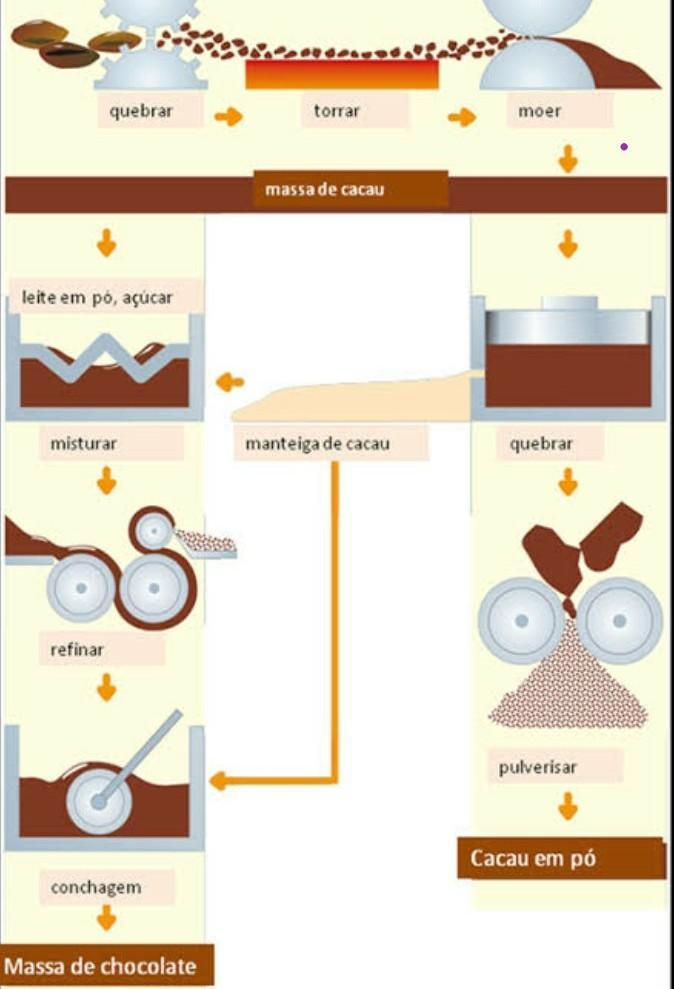
\includegraphics[scale=0.28]{../../Pictures/processocacau.jpg} 
\label{fig1}
\legend{Fonte: \cite{0}}
\end{center}
\end{figure}

O processamento do cacau é dividido em 11 fases majoritárias \cite{3}, são essas:

\begin{enumerate}
\item Colheita/Limpeza: O cacau é retirado cuidadosamente com uma faca para evitar qualquer injúria, após essa colheita cuidadosa acontece a limpeza do interior do cacau.
\item Fermentação: O processo de fermentação demora entre 36 a 72 horas e é um processo complexo e pouco entendido, mas está sendo desvendado com a tecnologia.
\item Secagem: Após a fermentação é necessário reduzir a humidade do cacau de aproximadamente 55$\%$ para 7,5$\%$, e para isso o cacau é deixado em plataformas de concreto para a secagem.
\item Torrefação: A torrefação varia de empresa para empresa e de região para região, pois está muito ligado ao tipo de saber desejado para aquele chocolate produzido, portanto não há um certo ou errado quando se fala do processo de torrefação.
\item Descasque: Separação da casca do grão propriamente dito.
\item Trituramento: Acontece a tritura desses grãos já separados
\item Alcalinização: Com o objetivo também de modificar o cheio e o gosto do chocolate, o processo consiste em misturar o cacau com uma solução aquosa alcalina específica e possivelmente colocando pressão no sistema ou até mesmo aumentando a temperatura.
\item Prensagem de licor: Adiciona-se pressão em um sistema com licor de cacau quente e o output é um bolo de cacau.
\item Moagem: Obtenção do licor propriamente dito a partir da prensagem
\item Manteiga de cacau: Outro material obtido a partir da prensagem.
\item Fabricação do chocolate: Processo de fabricação do chocolate.
\end{enumerate}


\newpage
\chapter{Balanço de Massa}
%\pagestyle{fancy}

\newpage
\chapter{Balanço de Energia}
%\pagestyle{fancy}

\newpage
\chapter{Conclusão}
%\pagestyle{fancy}


\newpage
\postextual

\bibliography{referencias}

%\begin{anexosenv}

%\chapter{Código utilizado no software EMSO}

%\begin{lstlisting}
%\end{lstlisting}

%\end{anexosenv}

\end{document}
